\section{Evaluation}
\label{sec:eval}

We evaluate RoboDSE at two levels. First, controlled execution ablations
establish how cross-chunk batching affects traffic and achievable inference
timing. Second, hardware exploration determines whether these improvements
change the resources required to satisfy latency and refresh constraints.
We then interpret representative timing choices using an empirical task-success
surface. This last analysis is a projection, not a new closed-loop validation.

\subsection{Experimental Setup and Methodology}
\label{sec:eval-setup}

\paragraph{Workload and hardware evaluation.}
The hardware workload models a VLM backbone and a flow-matching DiT action
expert with an action horizon of 16 and ten denoising steps. The implementation
uses two-byte weights, activations, and KV elements. Its structural dimensions
are estimates of the target model configuration rather than a verified
checkpoint extraction. Hardware evaluation combines compute timing templates,
calibrated memory-bandwidth models, and a periodic execution scheduler.
Estimated compute shapes and static SRAM assumptions retain their documented
limitations.

The frozen V7 population contains 39,928 retained hardware/mapping/period
identities, not 39,928 distinct physical designs. It includes LPDDR5, GDDR6,
and HBM2 configurations. We evaluate 22 constraint boxes
$B=(L_{\max},S_{\max})$, with $L_{\max}\in\{100,150,200,250,300\}$\,ms and
$S_{\max}\in\{50,75,100,150,200\}$\,ms, retaining $S_{\max}\leq L_{\max}$.
Table~\ref{tab:eval-setup} summarizes the evaluation settings. Selected timing
identities undergo 960-request checks after 192 warmup requests. These checks
establish scheduling consistency, not independent physical timing accuracy.

\begin{table}[t]
\centering
\caption{Evaluation settings and evidence scope.}
\label{tab:eval-setup}
\small
\begin{tabular}{@{}p{0.29\columnwidth}p{0.65\columnwidth}@{}}
\toprule
Item & Setting \\
\midrule
Workload & Estimated VLM/DiT structure; $H=16$; 10 denoising steps; 2-byte data \\
Core counts & 1, 2, 3, 4, 6, 8, 12, 16 \\
Shared SRAM & 8, 16, 32, 64 MB \\
Private SRAM & 512 or 2048 KB per core; feasibility-only timing assumption \\
Memory & LPDDR5, GDDR6, HBM2; conditional configurations flagged \\
Execution & Serial; pipelined $k=1,2,3$; batching on/off at $k=2,3$ \\
Timing search & Five relative-period factors: 1, 1.1, 1.25, 1.5, 2 \\
Task projection & 33 aggregate observations; linear interpolation inside the measured convex hull only \\
\bottomrule
\end{tabular}
\end{table}

\paragraph{Baselines and ablations.}
The batching mechanism ablation fixes physical hardware and the VLM/DiT
core split. Comparisons at matched $k$ isolate batching, whereas comparisons
across $k$ evaluate execution-organization tradeoffs. The fixed-split $k=1$
pipeline is not an independently optimized serial baseline.

For DSE, we compare three arms: the serial reference, joint exploration without
batching, and full RoboDSE. The no-batching arm retains serial execution,
the $k=1$ pipeline, and unbatched $k=2,3$ organizations. Full RoboDSE additionally
admits their batched counterparts. The resource comparison preserves the V7
reference convention: serial candidates satisfy $L\leq S_{\max}$, while joint
arms satisfy both actual $L\leq L_{\max}$ and $S\leq S_{\max}$. Resource
frontiers use core count and peak bandwidth; a sensitivity analysis additionally
includes total shared and private SRAM.

Because the original search used incumbent-based pruning, our main DSE
ablation performs fresh enumeration over all 576 hardware identities retained
by V7: nine memory/channel configurations, eight core counts, four shared-SRAM
sizes, and two private-SRAM sizes. Every legal core split and all five pipeline
organizations are searched, together with serial execution, without
incumbent pruning. The 16,416 configurations produce 82,070 accepted
mapping/period identities from 4,113 unique operation-template semantics.
Ten identities fail the unchanged periodic gate and are excluded. Equivalent
templates are reused, not treated as independent experimental repetitions.
The union of resource frontiers across comparisons and sensitivity settings
contains 510 identities, covered by 132 unique 960-request checks with
192 warmup requests. All pass, with maximum relative mean-$L/S$ discrepancy
$2.12\times10^{-11}$. The search remains restricted to the enumerated hardware,
mapping, and relative-period domain; it is not a continuous global optimum.

\paragraph{Task-performance interface.}
The imported task table provides 33 aggregate $(L,S)$ observations attributed
to $\pi_{0.5}$ with $H=16$ on LIBERO-Dynamic. Checkpoint, environment, and
delay-injection provenance remain to be verified, and per-speed trial
denominators are unavailable. We construct a piecewise-linear estimate
$\widehat{F}_{\tau}(L,S)$ inside the measured convex hull and abstain outside
it. Projected success values are descriptive estimates, not new task
measurements, confidence bounds, or independently validated recommendations.

\subsection{Effectiveness of Cross-Chunk Batching}
\label{sec:eval-batching}

\paragraph{Traffic reduction.}
Figure~\ref{fig:eval-batching}(a) shows the fixed-allocation LPDDR5 case with
four cores and 102.4\,GB/s peak bandwidth. Unbatched execution transfers
6.407\,GB of DiT data per request. Batching reduces this to 3.293\,GB at $k=2$
and 2.670\,GB at $k=3$, reductions of approximately 48.6\% and 58.3\%.
VLM traffic remains approximately unchanged, so total DRAM traffic decreases
from 11.188 to 8.074 and 7.451\,GB/request, respectively. These are total
traffic reductions of 27.8\% and 33.4\%. Under a fixed same-type energy-per-bit
coefficient, the traffic ratios equal estimated dynamic DRAM energy-per-request
ratios; they do not establish whole-chip energy or power reductions.

\begin{figure*}[t]
\centering
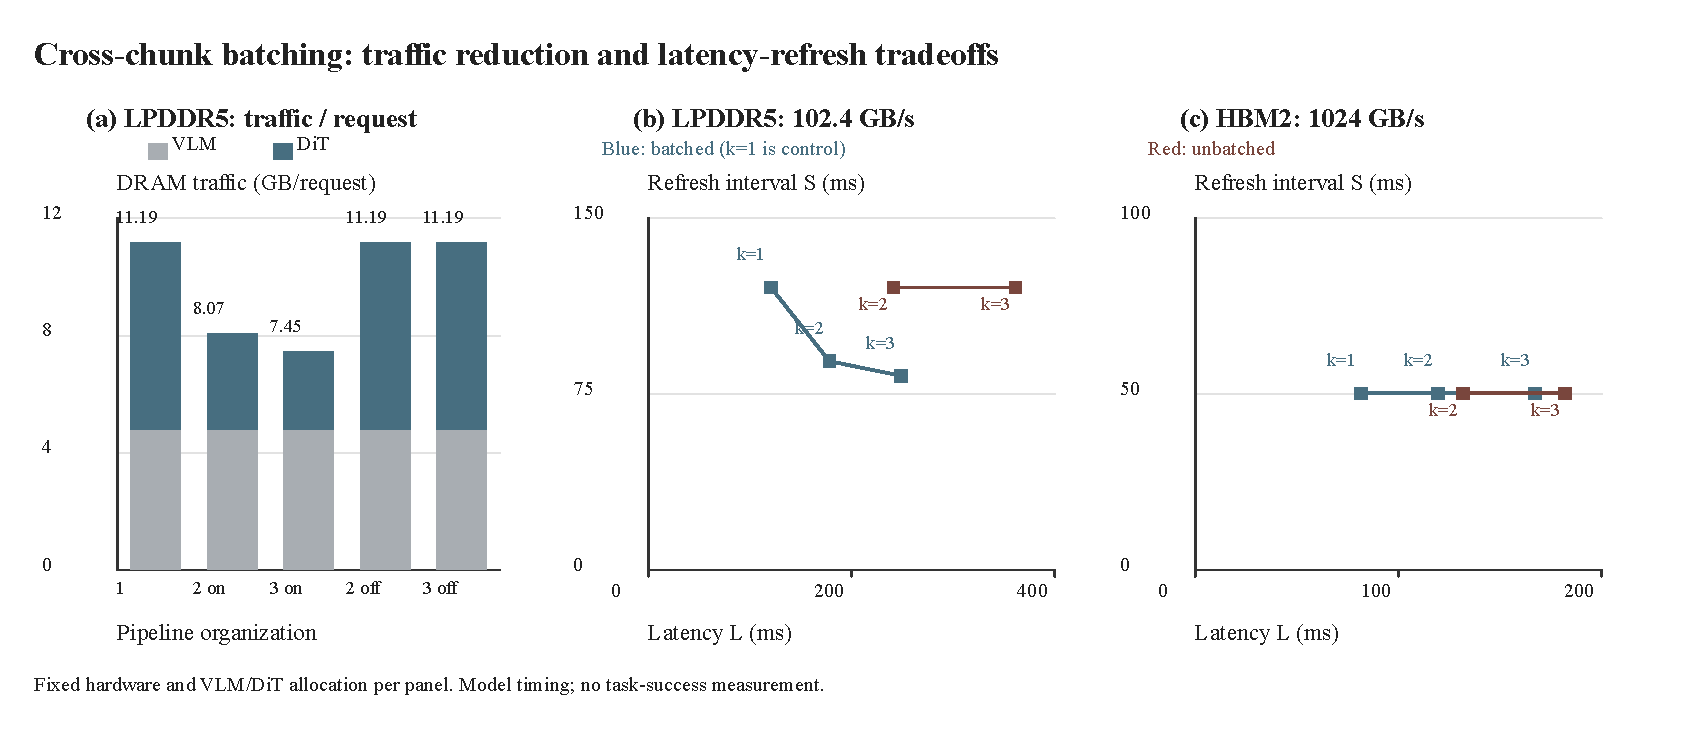
\includegraphics[width=\textwidth]{figure_1.pdf}
\caption{Cross-chunk batching under fixed hardware and core allocation.
(a) Per-request traffic on the low-bandwidth LPDDR5 platform.
(b) Its latency--refresh tradeoffs with and without batching.
(c) A high-bandwidth HBM2 counterexample. Connecting lines only guide the eye
between discrete organizations. These are hardware-model results, not task SR.}
\label{fig:eval-batching}
\end{figure*}

\paragraph{Timing improvement and execution tradeoffs.}
At fixed pipeline depth, batching improves both timing metrics
(Fig.~\ref{fig:eval-batching}(b)). At $k=2$, latency decreases from 241.09 to
178.16\,ms and refresh interval from 120.54 to 89.07\,ms. At $k=3$, latency
decreases from 361.63 to 248.48\,ms and refresh interval to 82.85\,ms.
Thus, the batching mechanism does not itself require trading latency for
refresh rate in these matched-$k$ comparisons.

Increasing pipeline depth introduces a separate tradeoff. The $k=1$ pipeline
control achieves $(L,S)=(120.55,120.54)$\,ms, while batched $k=2$ and $k=3$
achieve $(178.16,89.07)$ and $(248.48,82.85)$\,ms. The $k=2$ organization enters
Box$(200,100)$ by meeting its refresh bound while remaining within its latency
bound. The $k=3$ organization refreshes faster still, but exceeds this box's
latency limit.

\paragraph{Bottleneck dependence.}
The four-core HBM2 case in Fig.~\ref{fig:eval-batching}(c) provides
1024\,GB/s peak bandwidth. Its exposed-memory component is approximately
zero and its refresh interval is VLM-limited. Although traffic falls with
batching, $S$ remains approximately 50.26\,ms as $k$ increases, while latency
increases from 81.54\,ms at $k=1$ to 167.26\,ms at $k=3$. Batching therefore
provides more efficient execution options, but a fixed large $k$ is not
universally preferable. Hardware and execution organization must be selected
jointly for the required timing constraints.

\subsection{Joint Hardware and Execution-Organization Exploration}
\label{sec:eval-dse}

\paragraph{Resource-frontier improvements.}
Across the 22 boxes, full RoboDSE yields five strictly improved resource
frontiers, three extensions, and fourteen identical frontiers relative to the
serial reference (Fig.~\ref{fig:eval-dse}). Here, strict improvement means that
at least one alternative frontier vector strictly dominates a reference vector;
it does not mean every alternative design dominates every reference design.
Equality refers to resource-vector sets, not identical mappings. All 22 boxes
have nonempty reference and full-method resource frontiers in these tables.

The five strictly improved cases have $S_{\max}=50$\,ms. At six cores, a
representative comparison reduces peak bandwidth from 409.6 to 256.0\,GB/s,
a 37.5\% reduction. At eight cores, another comparison reduces bandwidth
from 256.0 to 204.8\,GB/s. A separate comparison at 256.0\,GB/s reduces the
core count from eight to six. These savings apply to their respective
matching conditions, not simultaneous reductions for a single design.

\paragraph{DSE-level no-batching ablation.}
In the fresh, unpruned enumeration, joint exploration without batching yields
the same resource frontiers as the serial reference in all 22 boxes.
Full RoboDSE therefore retains five strictly improved frontiers and three
extensions relative to this no-batching arm. These classification counts
also hold after excluding
conditional NoRefresh configurations and after including total SRAM as a
third Pareto dimension. Identical resource frontiers do not imply identical
$L,S$ values or the absence of all possible pipelining benefits.

\begin{figure*}[t]
\centering
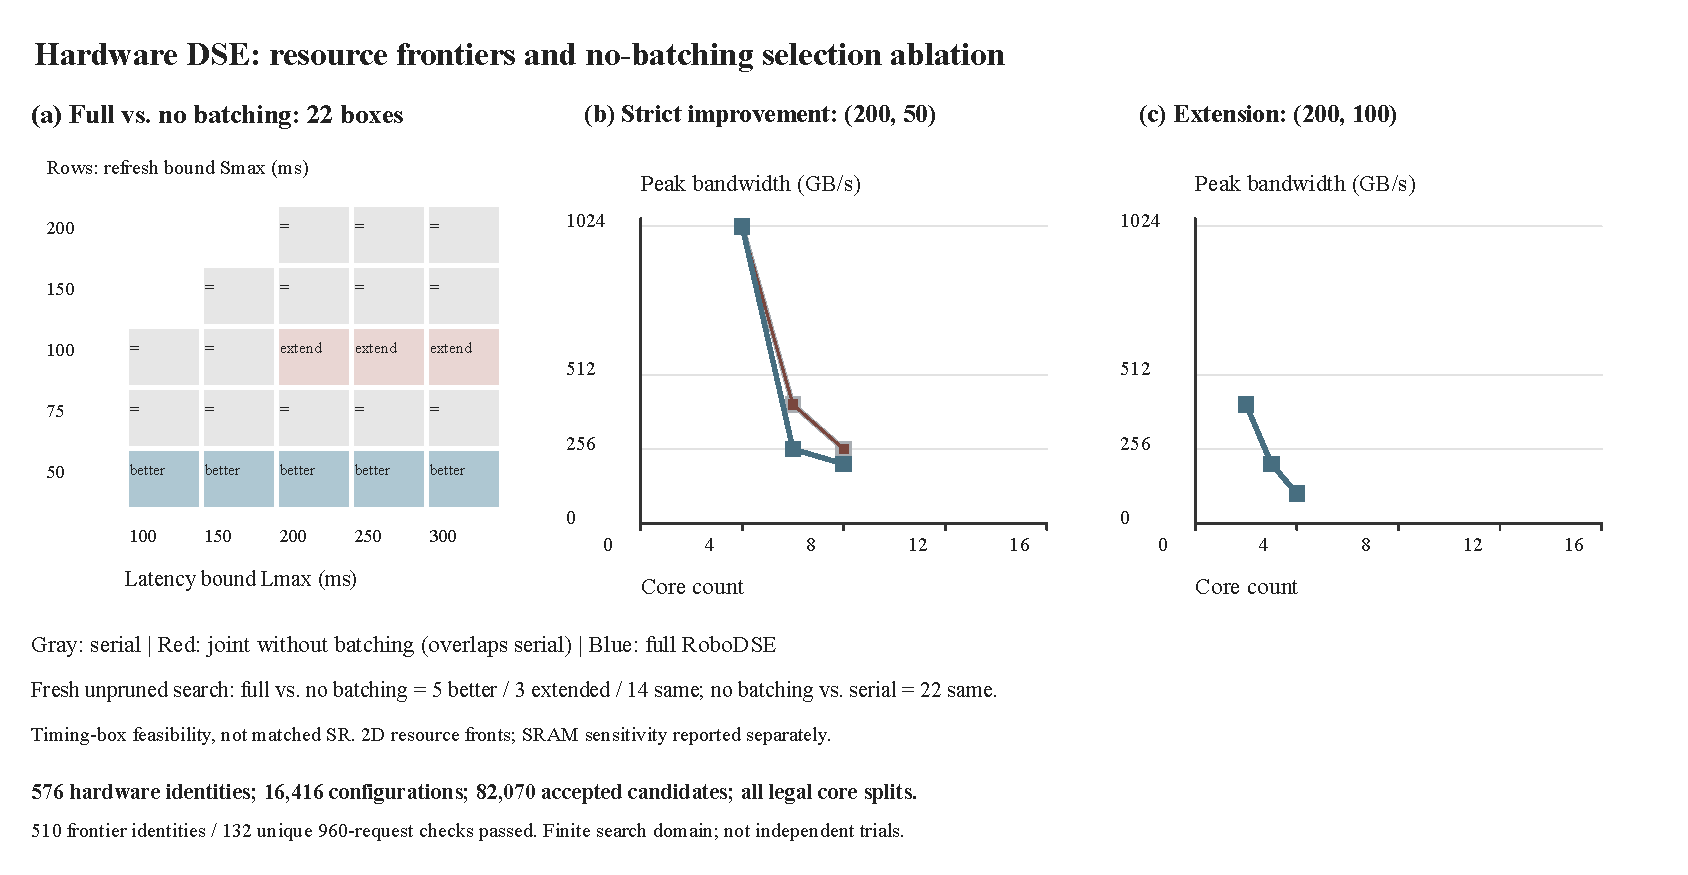
\includegraphics[width=\textwidth]{figure_2.pdf}
\caption{Hardware-resource exploration and no-batching ablation.
(a) Classification across the 22 timing boxes in the fresh unpruned search;
blank cells were not evaluated. (b) A strict-improvement example.
(c) A bandwidth--core tradeoff. Serial and no-batching resource frontiers
overlap. All legal core splits and five pipeline organizations are enumerated
on the same 576 retained hardware identities, with identical search rules.}
\label{fig:eval-dse}
\end{figure*}

An earlier matched-support filter of the pruned V7 population preserved the
five strict improvements but removed the three extensions. Such filtering
conditions on retained successful curves and cannot recover omitted mappings.
The fresh enumeration addresses that coverage limitation and reproduces all
three extensions without incumbent pruning.

\paragraph{Bandwidth--compute tradeoff.}
In the fresh enumeration, the serial reference for Box$(200,100)$
requires at least 204.8\,GB/s with three cores; a two-core alternative uses
409.6\,GB/s. The batched four-core design at 102.4\,GB/s halves the minimum
peak bandwidth at the expense of one additional core. This is a frontier
extension under common timing constraints, not strict dominance in all
resources. Box membership is not an empirical equal-success contour, so this
result is not presented as a matched-success resource reduction. Within the
four-core, 102.4\,GB/s subset, neither serial nor no-batching exploration has
a feasible point for this box, whereas batching admits
$(L,S)=(178.16,89.07)$\,ms.

\paragraph{Task-space interpretation.}
Of the frozen 39,928 candidate identities, 17,992 lie inside the measured
task-grid hull and 21,936 are excluded. Figure~\ref{fig:eval-task} projects
the fixed-allocation LPDDR5 trajectory onto this surface. The estimated mean
success rates are 46.76\%, 47.28\%, and 43.96\% for $k=1$, batched $k=2$,
and batched $k=3$, respectively. Thus, the shortest refresh interval does
not give the highest estimated success: the larger latency at $k=3$ can
outweigh the benefit of more frequent updates on this empirical surface.

\begin{figure*}[t]
\centering
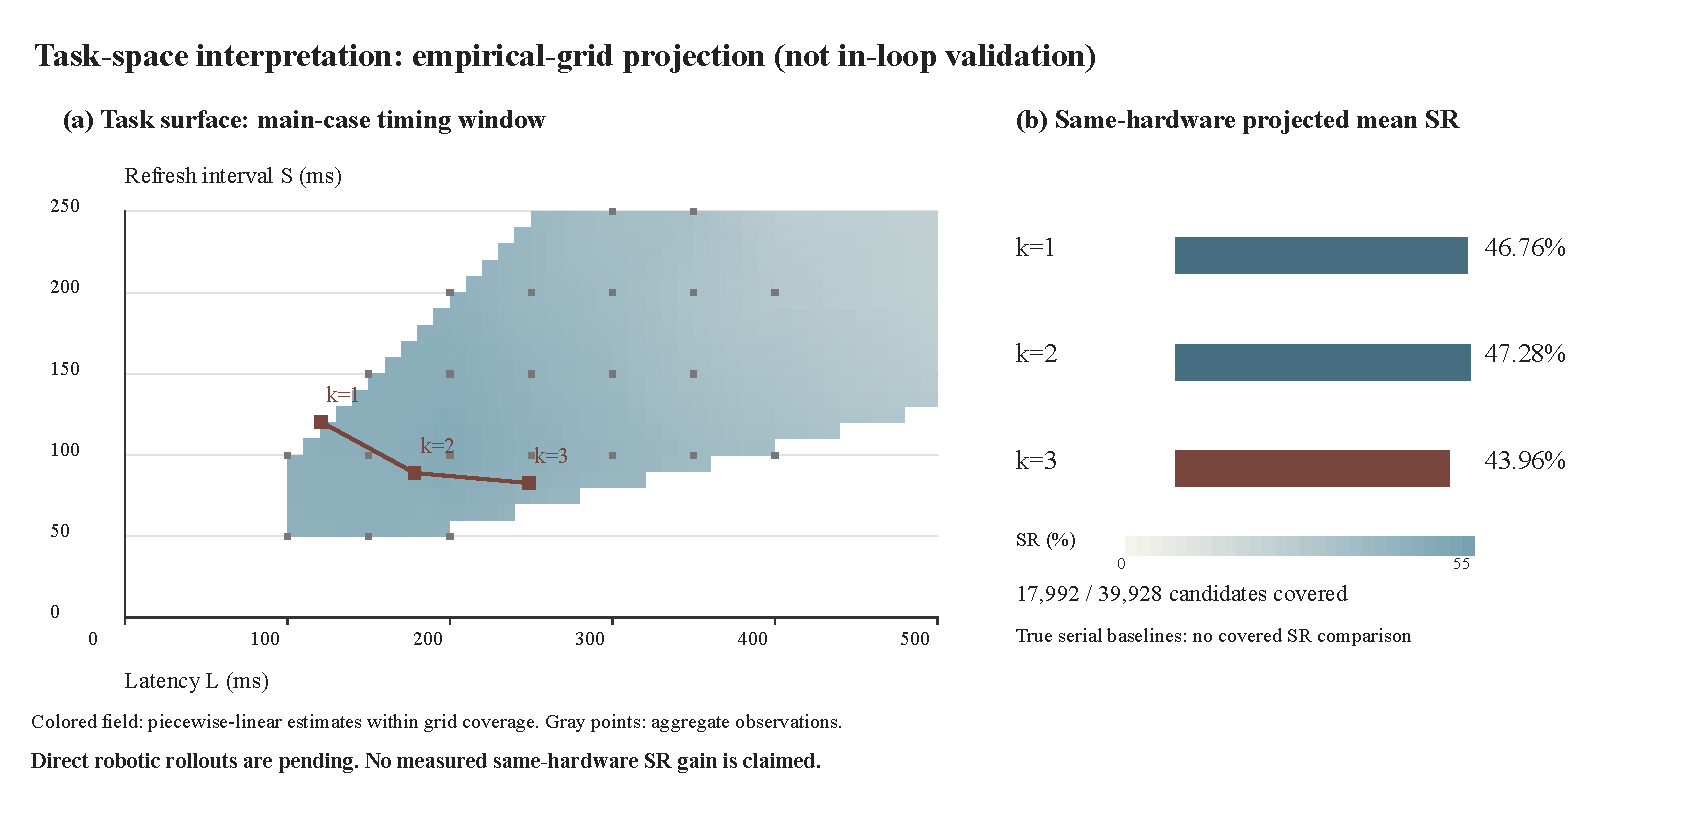
\includegraphics[width=\textwidth]{figure_3.pdf}
\caption{Task-space projection, not in-loop validation. (a) The main-case
timing window of the empirical surface, with aggregate observations and
fixed-allocation hardware trajectories. White regions have no displayed
interpolation. (b) Corresponding interpolated mean-success estimates.
No statistical confidence bounds or measured hardware-selection SR gains
are inferred from the aggregate table.}
\label{fig:eval-task}
\end{figure*}

The approximately 0.52-percentage-point difference between $k=1$ and $k=2$
is a conditional interpolation diagnostic, not a measured task improvement.
The 49.85\% observation at $(200,100)$\,ms is not assigned to the distinct
hardware point $(178.16,89.07)$\,ms. In the existing 264 refreshed-memory
same-hardware comparisons with covered alternatives, the independently chosen
minimum-latency serial baselines all lie outside the measured hull. We
therefore report no same-hardware DSE success gain. Selecting slower serial
baselines merely to obtain grid coverage would bias the comparison.

\paragraph{Cost sensitivity and remaining validation.}
In the frozen V7 sensitivity analysis, at central literature area coefficients,
none of the 22 boxes has a strictly
smaller globally selected task-aware area. Area remains a secondary
model-based sensitivity, not measured silicon evidence. Similarly,
cross-memory-type absolute energy rankings are not supported. Under the
existing deterministic bandwidth-stress scenarios, none of the 344
V7 strict-improvement task/box memberships reaches the threshold of feasibility
in at least 80\% of scenarios. This is a scenario fraction, not a probability
or confidence bound, and motivates bandwidth margin near feasibility limits.
These cost and stress analyses were not rerun over the fresh ablation domain.

The remaining task validation is to freeze representative designs and their
predicted $L,S$, reproduce those timings with matched observation and chunk
adoption semantics in the robotic simulator, and directly measure success
against the optimized serial and resource-reference designs. No such new
robotic rollouts are included here. The current primary findings are the
batching traffic/timing benefits and the resource-selection effects, including
the fresh, unpruned DSE-level no-batching ablation.
